\subsection{Probabilités}





\subsubsection{Axiomes de la théorie des probabilités}
\begin{center}
	$\left\{\begin{array}{LLL}
		P(E) &= 1\\
		P(A) &\geq 0&\forall A\subset E\\
		A \cap B &= \emptyset \Rightarrow P(A \cup B) = P(A)+P(B)
	\end{array}
	\right.$
\end{center}






\subsubsection{Probabilité indépendance}
Si $A$ et $B$ sont indépendants alors
\begin{itemize}
	\item $A$ et $\bar{B}$ sont indépendants ;
	\item $\bar{A}$ et $\bar{B}$ sont indépendants ;
	\item $\bar{A}$ et $B$ sont indépendants.
\end{itemize}






\subsubsection{Probabilité conditionnelle et indépendance}
Probabilité conditionnelle de $A$ sous la condition $B$ ("sachant $B$") :
$$P(A|B)=\frac{P(A \cap B)}{P(B)}$$
Si A est indépendant de $B$ :
	$\left\{\begin{array}{LL}
		P(A \cap B)&=P(A)P(B)\\
		P(A|B)&=P(A)\\
		P(B|A)&=P(B)
	\end{array}
\right.$
\begin{flushright}
Une des propriétés des 3 suffit.
\end{flushright}
\paragraph{Démonstration}
La probabilité conditionnelle respecte les axiomes de la théorie des probabilités
\begin{center}
	$\begin{array}{LCCL}
		P(E|A) &=& \dfrac{P(E\cap A)}{P(A)} = \dfrac{P(A)}{P(A)}&=1\\
		P(B|A) &=& \dfrac{P(B\cap A)}{P(A)}&\geq0\\
		X\cap Y\neq\emptyset &\Rightarrow& P(X\cup Y |A)\\
		&&\dfrac{P((X\cup Y)\cap A)}{P(A)}\\
		&&\dfrac{P((X\cap A)\cup (Y\cap A))}{P(A)}\\
		&&\dfrac{P(X\cap A) + (Y\cap A)}{P(A)}\\
		&&\dfrac{P(X|A)P(A) + P(Y|A)P(A)}{P(A)}\\
		&&P(X|A) + P(Y|A)\\
	\end{array}$
\end{center}






\subsubsection{Probabilité conditionnelle inverse et indépendant}
$$P(A|B) = P(A|\bar{B})$$
\paragraph{Démonstration}
\begin{center}
	$\begin{array}{CCC}
		P(A|B)                   &=& P(A|\bar{B})\\
		\dfrac{P(A\cap B)}{P(B)} &=& \dfrac{P(A\cap\bar{B})}{P(\bar{B})}\\
		\dfrac{P(A) P(B)}{P(B)}  &=& \dfrac{P(A)P(B)}{P(\bar{B})}\\
		P(A)                     &=& P(A)\\
	\end{array}$
\end{center}








\subsubsection{Formule de Bayes}
Cette formule est utilisée dans le cas où un évènement $B$ peut survenir à cause d'évènement $A_i$ incompatibles. Par exemple : une pièce défectueuse fabriquée par plusieurs machines différentes.
\begin{center}
	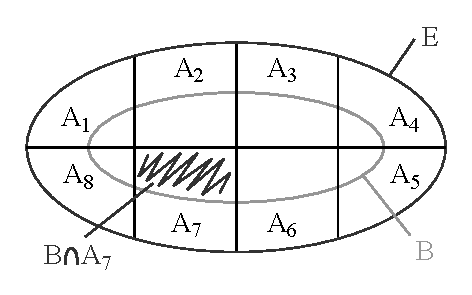
\includegraphics[width=0.3\textwidth]{images/formule-de-bayes} 
\end{center}
\begin{center}
	$\begin{array}{CCCCCCCCC}
		B    & = & (A_1 \cap B)      & \cup & (A_2 \cap B)      & \cup & \dots & \cup & (A_m \cap B)\\
		P(B) & = & P(A_1 \cap B)     & +    & P(A_2 \cap B)     & +    & \dots & +    & P(A_m \cap B)\\
		     & = & P(B | A_1) P(A_1) & +    & P(B |A_2) P(A_2) & +    & \dots & +    & P(B |A_m) P(A_m)
	\end{array}$
\end{center}

$$\boxed{P(A_k|B)=\frac{A_k \cap B}{P(B)}=\frac{P(B|A_k)P(A_k)}{\displaystyle\sum_{j=1}^{m}P(B|A_j)P(A_j)}}$$